\documentclass[tikz]{standalone}

\begin{document}
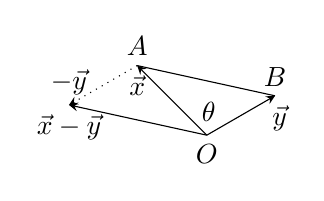
\begin{tikzpicture}
  \draw[variable=\r, ->, >=stealth, domain=0:1.25]
  plot( {\r*cos(135)}, {\r*sin(135)} ) node[above] {\(A\)}
  node[below] {\(\vec{x}\)};	
  \draw[variable=\r, ->, >=stealth, domain=0:1]
  plot( {\r*cos(30)}, {\r*sin(30)} ) node[above] {\(B\)} node[below] {\(\ \vec{y}\)};
  \node[below] at (0,0) {\(O\)}; 
  \draw[variable=\r, ->, >=stealth, domain=0:1, dotted]
  plot( {-0.8838834765 + \r*cos(-150)}, {0.8838834765 + \r*sin(-150)} ) node[above] {\(-\vec{y}\)};
  \draw[->,>=stealth] (0,0)--(-1.749908880,0.3838834765) node[below] {\(\vec{x}-\vec{y}\)};
  \draw (0.8660254040,0.5)--(-0.8838834765,0.8838834765);
  \node[above] at (0.025,0.05) {\(\theta\)};
\end{tikzpicture}
\end{document}
